\section{平稳分布}
\label{sec:graph-walk-stationary}

走了很多步以后，分布会不会停在某个固定形状上？如果给每个顶点分配一定的概率质量，使得一步转移后各点的质量恰好不变，这份分布就叫平稳分布。我们先用四点路径的具体算例看到这样的分布确实存在，再回到一般的无向图推导它的形式。

在四点路径上，试着给每条边的每个端点各分出$1/6$的质量。三条边共分出六份，各顶点收到的份数与自身的邻边数一致：端点$1$和$4$各收到一份，中间的$2$和$3$各收到两份。于是初始质量为$(1,2,2,1)/6$。

现在看一步转移。端点$1$的一份质量全部送给$2$。中间顶点$2$有两份质量，一份送给$1$，另一份送给$3$。边$23$和$34$上的情况也是类似的对称交换。图~\ref{fig:graph-walk-stationary-edge-balance}标出了每条边上的两笔对向转移。任取一个顶点，加起来的流入恰好等于加起来的流出。一步之后各点质量都没有变化。

\begin{BookInlineFigure}
\centering
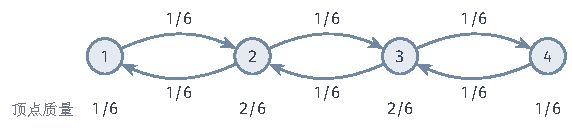
\includegraphics[width=96.936mm]{figures/03-graphs/05-matrices-and-spectra/tikz/walk-examples/stationary-edge-balance.pdf}
\caption{四顶点单位权路径的平稳概率及一步转移量。节点下方是原有质量，同一条边的两个方向各送出$1/6$。}
\label{fig:graph-walk-stationary-edge-balance}
\end{BookInlineFigure}

\begin{definition}[平稳分布]
\label{def:graph-walk-stationary}
若非负行向量$\bm{\pi}$满足$\sum_i\pi_i=1$且
\begin{equation}
\bm{\pi}\bm{P}=\bm{\pi},
\label{eq:graph-walk-stationary}
\end{equation}
则称$\bm{\pi}$是转移矩阵$\bm{P}$的\term{平稳分布}（stationary distribution）。
\end{definition}

上面四点路径的例子提示了一种做法：让每个顶点持有与其度成正比的质量。在一般的加权无向图上，令
\[
\pi_i=\frac{d_i}{\operatorname{vol}(V)}.
\]
下面验证这确实是一个平稳分布。

\paragraph{详细平衡}

考虑一条边$\{i,j\}$上的双向概率流。从$i$送往$j$的流量是当前在$i$的概率乘以从$i$到$j$的转移概率，
\[
\pi_i P_{i,j}=\frac{d_i}{\operatorname{vol}(V)}\cdot\frac{w_{i,j}}{d_i}
=\frac{w_{i,j}}{\operatorname{vol}(V)}.
\]
右边只含边权$w_{i,j}$，与方向无关。交换$i,j$后结果不变，因为$w_{i,j}=w_{j,i}$。这就是说，每条边上从两端送出的概率流相等。这个性质称为\term{详细平衡}（detailed balance）。

既然每条边的双向流已经抵消，对起点$i$求和后，流入$j$的总量自然等于$j$原有的质量$\pi_j$。因此按度分配的分布确实平稳。详细平衡是一个比平稳方程更强的条件：后者只要求每个顶点的总流入等于总流出，前者要求每条边上都各自平衡。

\paragraph{唯一性}

接下来说明连通无向图的平稳分布唯一。

\begin{theorem}[无向连通图的平稳分布]
\label{thm:graph-walk-stationary-uniqueness}
正权支撑连通的有限无向图的转移矩阵$\bm P$有唯一的平稳分布，且$\pi_i=d_i/\operatorname{vol}(V)$。
\end{theorem}

\begin{proof}
设$\bm{q}$是任意一个平稳分布，满足$\bm{q}\bm{P}=\bm{q}$。将等式写成$\bm{q}\bm{D}^{-1}\bm{W}=\bm{q}$，两边转置得
\[
\bm{W}\bm{D}^{-1}\bm{q}^\top=\bm{q}^\top.
\]
这里用了$\bm{W}$对称和$\bm{D}^{-1}$为对角矩阵。

令$\bm{y}=\bm{D}^{-1}\bm{q}^\top$，即$y_i=q_i/d_i$。等式右边的$\bm{q}^\top$可以写成$\bm{D}\bm{y}$，于是
\[
(\bm{D}-\bm{W})\bm{y}=\bm{0}.
\]
左边正是组合拉普拉斯$\bm{L}$作用于$\bm{y}$。第~\ref{chap:graph-laplacian-matrix}章指出，连通图的拉普拉斯零空间由常向量张成。这意味着$y_i=q_i/d_i$对所有$i$取相同的值。由总质量$\sum_i q_i=1$确定这个常数为$1/\operatorname{vol}(V)$，于是
\begin{equation}
\pi_i=\frac{d_i}{\operatorname{vol}(V)}.
\label{eq:graph-walk-stationary-degrees}
\end{equation}
\end{proof}

\paragraph{不连通与收敛的区别}

若图有多个正权连通分量，每个分量可以独立保有自己的概率质量。取各分量平稳分布的任意凸组合仍然平稳，因此唯一性不再成立。孤点上的点质量也可以保留——在停留规则下它已经平稳。

回到只有一条边的两点图。它只有一个正权分量，平稳分布唯一，为$(1/2,1/2)$。但如果从其中一个顶点出发，棋子每一步切换顶点，分布在$(1,0)$与$(0,1)$之间交替，始终不收敛。平稳分布的唯一性回答了"哪些分布保持不变"，至于任意初态能否到达它，还需要检查矩阵幂的行为。
